\section{Implementation Details}


This section provides an overview of how the Safety Annex is related to AADL, AGREE, and the JKind model checker.  The Safety Annex is written in Java as a plug-in for the OSATE AADL toolset, which is built on Eclipse.  It is not designed as a stand-alone extension of the language, but works with behavioral contracts specified AGREE annex and associated tools.  AGREE allows assume-guarantee behavioral contracts to be added to AADL components.  The language used for contract specification is based on the Lustre dataflow language~\cite{Halbwachs91:IEEE}. 

The organization of these interactions  is shown in Figure~\ref{fig:plugin-arch}. The AADL file is annotated with AGREE contracts which creates the nominal model.This nominal model is parsed and sent to JKind in order to perform formal verification. If the Safety Annex is also annotated within this model, this creates the extended (fault) model. When desired, the user can run ``Perform Safety Analysis'' within the Osate environment. This creates an extension point where the Safety Analysis informaiton is added into the AGREE model before getting passed to JKind for analysis. In either case, the JKind verification result is returned and displayed to the user in the Osate environment. For more information about this process, see the Safety Annex Users Guide or the technical report~\cite{amaseRepo,SATechReport}.

\begin{figure}
\begin{center}
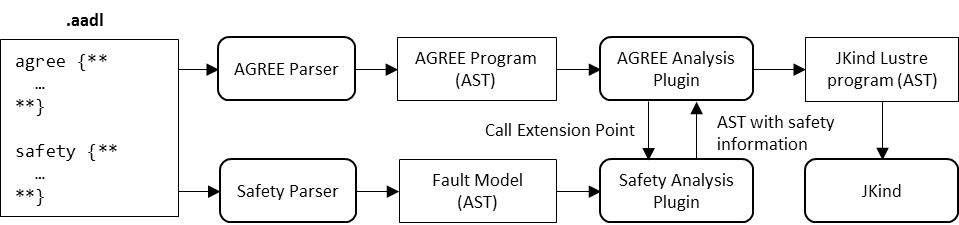
\includegraphics[width=.9\textwidth]{images/arch.png}
\end{center}
\vspace{-0.2in}
\caption{Safety Annex Plug-in Design}
\label{fig:plugin-arch}
\end{figure}

AGREE contracts are used to define the nominal behaviors of system components as {\em guarantees} that hold when {\em assumptions} about the values the component's environment are met.  The Safety Annex extends these contracts to allow faults to modify the behavior of component inputs and outputs.  To support these extensions, AGREE implements an Eclipse extension point interface that allows other plug-ins to modify the generated abstract syntax tree (AST) prior to its submission to the solver.  If the Safety Annex is enabled, these faults are added to the AGREE contract and, when triggered, override the nominal guarantees provided by the component.  An example of a portion of an initial AGREE node and its extended contract is shown in Figure~\ref{fig:comp}.  The \texttt{\_\_fault} variables and declarations are added to allow the contract to override the nominal behavioral constraints (provided by guarantees) on outputs.  In the Lustre language, \texttt{assertion}s are constraints that are assumed to hold in the transition system.

\begin{figure}
\vspace{-0.1in}
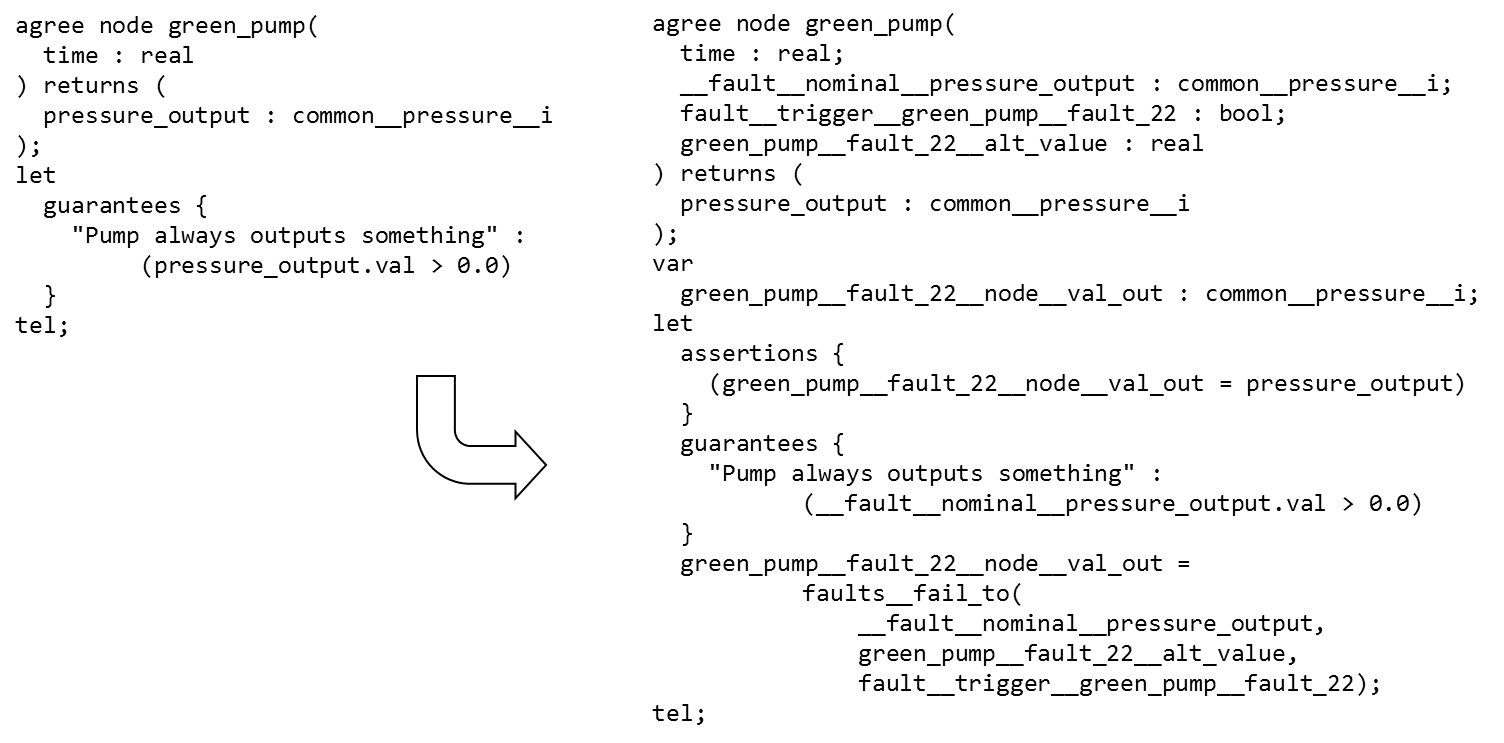
\includegraphics[width=\textwidth]{images/sample_code.png}
\vspace{-0.3in}
\caption{Nominal AGREE node and its extension with faults}
\label{fig:comp}
\end{figure}

An annotation in the AADL model determines the fault hypothesis.  This may specify either a maximum number of faults that can be active at any point in execution (typically one or two), or that only faults whose probability of simultaneous occurrence is above some probability threshold should be considered.  In the former case, we assert that the sum of the true {\em fault\_\_trigger} variables is below some integer threshold.  In the latter, we determine all  combinations of faults whose probabilities are above the specified probability threshold, and describe this as a proposition over {\em fault\_\_trigger} variables.

Once augmented with fault information, the AGREE model follows the standard AGREE translation path to the model checker JKind~\cite{2017arXiv171201222G}, an infinite-state model checker for safety properties.  The augmentation includes traceability information so that when counterexamples are displayed to users, the active faults for each component are visualized.



